\documentclass[12pt]{article}

%% FONTS
%% To get the default sans serif font in latex, uncomment following line:
 \renewcommand*\familydefault{\sfdefault}
%%
%% to get Arial font as the sans serif font, uncomment following line:
%% \renewcommand{\sfdefault}{phv} % phv is the Arial font
%%
%% to get Helvetica font as the sans serif font, uncomment following line:
% \usepackage{helvet}
\usepackage[small,bf,up]{caption}
\renewcommand{\captionfont}{\footnotesize}
\usepackage[left=1in,right=1in,top=1in,bottom=1in]{geometry}
\usepackage{graphics,epsfig,graphicx,float,subfigure,color}
\usepackage{amsmath,amssymb,amsbsy,amsfonts,amsthm}
\usepackage{url}
\usepackage{boxedminipage}
\usepackage[sf,bf,tiny]{titlesec}
 \usepackage[plainpages=false, colorlinks=true,
   citecolor=blue, filecolor=blue, linkcolor=blue,
   urlcolor=blue]{hyperref}
\usepackage{enumitem}
\usepackage{verbatim}
\usepackage{tikz,pgfplots}

\newcommand{\todo}[1]{\textcolor{red}{#1}}
% see documentation for titlesec package
% \titleformat{\section}{\large \sffamily \bfseries}
\titlelabel{\thetitle.\,\,\,}

\newcommand{\bs}{\boldsymbol}
\newcommand{\alert}[1]{\textcolor{red}{#1}}
\setlength{\emergencystretch}{20pt}

\begin{document}

\begin{center}
  \vspace*{-2cm}
{\small MATH-GA 2012.001 and CSCI-GA 2945.001, B.~Peherstorfer (Courant NYU); adapted from G.~Stadler}\end{center}
\vspace*{.5cm}
\begin{center}
\large \textbf{%%
Spring 2022: Advanced Topics in Numerical Analysis: \\
High Performance Computing \\
Assignment 2 (due Mar.\ 21, 2022) }
\end{center}


% ****************************

\noindent {\bf Handing in your homework:} Please create a Git
repository on Github  to hand in your homework.  If you
choose your repository to be private, please give Melody and Cai (who are helping with grading) read access to the repo (Melody's username is 
\texttt{melodyshih} and Cai's is \texttt{caim-d}).
The repository should contain the source
files, as well as a Makefile.
To hand in your homework, please email me and Melody together a
single message with the location of your repo. Generate a \texttt{hw2}
directory in this repo, which contains all the source code and a
short \texttt{.txt} or \LaTeX\ file that answers the questions/reports
timings from this assignment. Alternatively, you can hand in a sheet
with the answers/timings that also specifies the location of your
repo.  To check if your code runs, we will type the following
commands\footnote{Since we will partially automize this, make sure
  this will work for the code you hand in.}:
\begin{verbatim}
git clone YOURPATH/YOURREPO.git
cd YOURREPO/hw2/
make
./MMult1
./val_test01_solved
./val_test02_solved
./omp_solved2
...
./omp_solved6
./jacobi2D-omp
./gs2D-omp
\end{verbatim}
The folder homework02 in the git repository \url{https://github.com/pehersto/HPCSpring2022}
contains the matrix-matrix multiplication code you can start with, and
the buggy code examples needed for this homework.\footnote{And
  yes, these examples can also be found on the web---but for your own
  sake, please try to understand what's going on and try to find the
  bugs.} For an overview over OpenMP, you can use the material and
examples from class and the official documentation for the OpenMP
Standard
5.0.\footnote{\url{http://www.openmp.org/specifications/}}
\\[1ex]
%
% ****************************
\begin{enumerate}
% --------------------------
 \item {\bf Finding Memory bugs.}  The homework repository contains
   two simple programs that contain bugs. Use valgrind to find these
   bugs and fix them. Add a short comment to the code describing what
   was wrong and how you fixed the problem. Add the solutions to your
   repository using the naming convention
   \texttt{val\_test01\_solved.cpp, val\_test02\_solved.cpp}, and use
   the Makefile to compile the example problems.

  \item {\bf Optimizing matrix-matrix multiplication.} In this
    homework you will optimize the matrix-matrix multiplication code
    from the last homework using blocking. This increases the
    computational intensity (i.e., the ratio of flops per access to
    the slow memory) and thus speed up the implementation
    substantially. The code you can start with, along with further
    instructions are in the source file
    \texttt{MMult1.cpp}. Specifying what machine you run on, hand in
    timings for various matrix sizes obtained with the blocked version
    and the OpenMP version of the code.

\item {\bf Finding OpenMP bugs.}  The homework repository contains five
  OpenMP problems that contain bugs. These files are in C, but they
  can be compiled with the C++ compiler. Try to find these bugs and fix
  them. Add a short comment to the code describing what was wrong and
  how you fixed the problem. Add the solutions to your repository
  using the naming convention
  \texttt{omp\_solved}\{2,\ldots\}\texttt{.c}, and provide a Makefile
  to compile the fixed example problems.

\item {\bf OpenMP version of 2D Jacobi/Gauss-Seidel smoothing.}
  Implement first a serial and then an OpenMP version of the
  two-dimensional Jacobi and Gauss-Seidel smoothers. This is similar
  to the problem on the first homework assignment, but for the unit
  square domain $\Omega=(0,1)\times (0,1)$. For a given function
  $f:\Omega\to \mathbb R$, we aim to find $u:\Omega\to \mathbb R$ such
  that
  \begin{equation}\label{eq:Laplace}
    -\Delta u := -(u_{xx}+u_{yy}) = f \text { in } \Omega,
  \end{equation}
  and $u(x,y) = 0$ for all boundary points $(x,y)\in \partial\Omega :=
  \{(x,y) : x=0 \text{ or } y=0 \text{ or } x=1 \text{ or } y=1\}$.
  We go through analogous arguments
  as in homework 1, where we used finite differences to discretize the
  one-dimensional version of \eqref{eq:Laplace}. In two dimensions, we
  choose the uniformly spaced points
  $\{(x_i,y_j)=(ih,jh):i,j=0,1,\ldots,N,N+1\}\subset [0,1]\times
  [0,1]$, with $h = 1/(N+1)$, and approximate $u(x_i,y_j)\approx
  u_{i,j}$ and $f(x_i,y_j)\approx f_{i,j}$, for $i,j=0,\ldots,
  N+1$; see Figure~\ref{fig} (left).  Using Taylor expansions as in
  the one-dimensional case results in
  $$
  -\Delta u(x_i,y_j) = \frac{-u(x_i\!-\!h,y_j) \!-\! u(x_i,y_j\!-\!h)  \!+\! 4u(x_i,y_j) \!-\!
    u(x_i\!+\!h,y_j) \!-\!  u(x_i,y_j\!+\!h)}{h^2} + \text{h.o.t.},
  $$
  where h.o.t.\ stands for a remainder term that is of higher order in
  $h$, i.e., becomes small as $h$ is decreased. Hence, we approximate the
  Laplace operator at a point $(x_i,y_j)$ as follows:
  $$
-\Delta  u_{ij} = \frac{-u_{i-1,j} - u_{i,j-1} + 4u_{ij} - u_{i+1,j} -
    u_{i,j+1} }{h^2}.
  $$ This results in a linear system, that can again be written as
  $A\bs u = \bs f$,
  where
  \begin{align*}
    \bs u&=(u_{1,1},u_{1,2},\ldots,u_{1,N},u_{2,1},u_{2,2},\ldots,u_{N,N-1},u_{N,N})^\top,\\
    \bs f&=(f_{1,1},f_{1,2},\ldots,f_{1,N},f_{2,1},f_{2,2},\ldots,f_{N,N-1},f_{N,N})^\top.
  \end{align*}
  Note that the points at the boundaries are not included, as we know
  that their values to be zero.
\begin{figure}\centering
  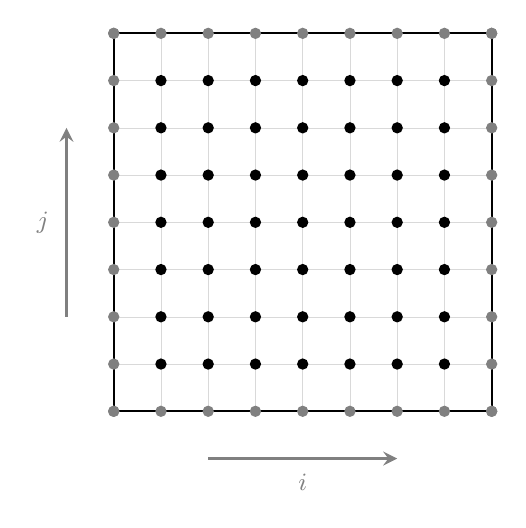
\begin{tikzpicture}[scale=0.6]
    \draw[step=1cm, gray!30!white, very thin] (0,0) grid (8,8);
    \draw[thick] (-0,0) -- (8,0);
    \draw[thick] (0,0) -- (0,8);
    \draw[thick] (0,8) -- (8,8);
    \draw[thick] (8,0) -- (8,8);
    % inner points
    \foreach \x in {1,...,7}
    \foreach \y in {1,...,7}
    \fill[black] (\x,\y) circle (0.12cm);
    \foreach \x in {0,8}
    \foreach \y in {0,...,8}
    \fill[gray] (\x,\y) circle (0.12cm);
    \foreach \y in {0,8}
    \foreach \x in {0,...,8}
    \fill[gray] (\x,\y) circle (0.12cm);
    \draw[->,>=stealth,very thick,gray] (-1,2) -> (-1,6);
    \node at (-1.5,4) {\small\textcolor{gray}{ $j$}};
    \draw[->,>=stealth,very thick,gray] (2,-1.) -> (6,-1.);
    \node[rotate=0] at (4,-1.5) {\small\textcolor{gray}{ $i$}};
\end{tikzpicture} \hspace{5ex}
  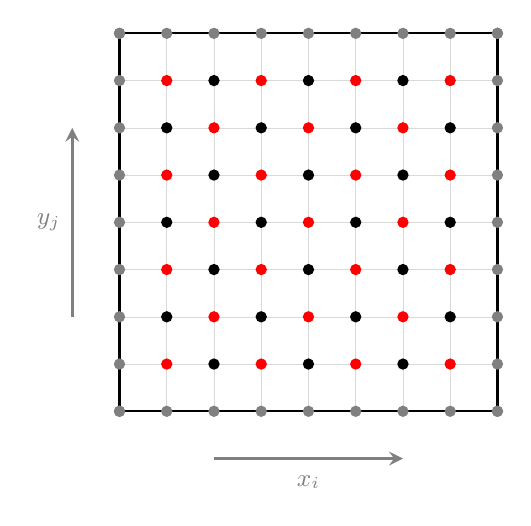
\begin{tikzpicture}[scale=0.6]
    \draw[step=1cm, gray!30!white, very thin] (0,0) grid (8,8);
    \draw[thick] (-0,0) -- (8,0);
    \draw[thick] (0,0) -- (0,8);
    \draw[thick] (0,8) -- (8,8);
    \draw[thick] (8,0) -- (8,8);
    % inner points
    \foreach \x in {1,3,...,7}
    \foreach \y in {2,4,...,7}
    \fill[black] (\x,\y) circle (0.12cm);
    \foreach \x in {2,4,...,7}
    \foreach \y in {1,3,...,7}
    \fill[black] (\x,\y) circle (0.12cm);
    \foreach \x in {1,3,...,7}
    \foreach \y in {1,3,...,7}
    \fill[red] (\x,\y) circle (0.12cm);
    \foreach \x in {2,4,...,7}
    \foreach \y in {2,4,...,7}
    \fill[red] (\x,\y) circle (0.12cm);
    \foreach \x in {0,8}
    \foreach \y in {0,...,8}
    \fill[gray] (\x,\y) circle (0.12cm);
    \foreach \y in {0,8}
    \foreach \x in {0,...,8}
    \fill[gray] (\x,\y) circle (0.12cm);
    \draw[->,>=stealth,very thick,gray] (-1,2) -> (-1,6);
    \node at (-1.5,4) {\small\textcolor{gray}{ $y_j$}};
    \draw[->,>=stealth,very thick,gray] (2,-1.) -> (6,-1.);
    \node[rotate=0] at (4,-1.5) {\small\textcolor{gray}{ $x_i$}};
\end{tikzpicture}
\caption{Sketch of discretization points for unit square for
  $N=7$. Left: Dark points are unknowns, grey points at the boundary
  are zero. Right: red-black coloring of unknowns. Black and red
  points can be updated independently in a Gauss-Seidel
  step.\label{fig}}
\end{figure}
Similarly to the one-dimensional case, the resulting Jacobi update for
solving this linear system is
\begin{equation*}
  u_{i,j}^{k+1} = \frac{1}{4}\left(h^2 f_{i,j} + u^k_{i-1,j}+ u^k_{i,j-1}+ u^k_{i+1,j}+ u^k_{i,j+1} \right),
\end{equation*}
   and the Gauss-Seidel update is given by
  \begin{equation*}
  u_{i,j}^{k+1} = \frac{1}{4}\left(h^2 f_{i,j} + u^{k+1}_{i-1,j}+
  u^{k+1}_{i,j-1}+ u^k_{i+1,j}+ u^k_{i,j+1} \right),
  \end{equation*}
  where it depens on the order of the unknowns which entries on the
  right hand side are based on the $k$th and which on the $(k+1)$st
  iteration. The above update formula is for lexicographic ordering of
  the points, i.e., we sweep from left to right first and go row by
  row from the bottom to the top.
  Usually, as in the one-dimensional case, one use a single
  vector $\bs u$ of unknows, which are overwritten and the latest
  available values are used.

  As can be seen, the update at the $(i,j)$th point in the Gauss-Seidel
  smoother depends on previously updated points. This dependence makes
  it difficult to parallelize the Gauss-Seidel algorithm. As a remedy,
  we consider a variant of Gauss-Seidel, which uses \emph{red-black
    coloring} of the unknowns. This amounts to ``coloring'' unknowns as
  shown in Figure~\ref{fig} (right), and into splitting each
  Gauss-Seidel iteration into two sweeps: first, one updates all black
  and then all the red points (using the already updated red
  points). The point updates in the red and black sweeps are
  independent from each other and can be
  parallelized using OpenMP.\footnote{Depending on the discretization and the
    dimension of the problem, one might require more than two colors
    to ensure that updates become independent from each other and
    allow for parallelism. Efficient coloring for unstructured meshes
    with as little colors as possible is a difficult research
    question.}
  To detail the equations, this become the following update, where colors of the
  unknowns correspond to the colors of points in the figure, i.e.,
  first we update all red points, i.e., $(i,j)$ corresponds to indices
  for red points,
  \begin{equation*}
  \textcolor{red}{u_{i,j}^{k+1}} = \frac{1}{4}\left(h^2 f_{i,j} + u^{k}_{i-1,j}+
  u^{k}_{i,j-1}+ u^k_{i+1,j}+ u^k_{i,j+1} \right),
  \end{equation*}
  and then we update all black points, i.e.,  $(i,j)$ are indices
  corresponding to black points:
  \begin{equation*}
    \textcolor{black}{u_{i,j}^{k+1}} = \frac{1}{4}\left(h^2 f_{i,j} + \textcolor{red}{u^{k+1}_{i-1,j}}+
    \textcolor{red}{u^{k+1}_{i,j-1}}+ \textcolor{red}{u^{k+1}_{i+1,j}}+
    \textcolor{red}{u^{k+1}_{i,j+1}} \right).
  \end{equation*}
  At the end, every point is on level $(n+1)$ and we repeat.
    \begin{itemize}
  \item Write OpenMP implementations of the Jacobi and the
    Gauss-Seidel method with red-black coloring, and call them
    \texttt{jacobi2D-omp.cpp} and \texttt{gs2D-omp.cpp}. Make sure your
    OpenMP codes also compile without OpenMP compilers using
    preprocessor commands (\texttt{\#ifdef \_OPENMP}) as shown in
    class.
  \item Choose the right hand side $f(x,y)\equiv 1$, and report
    timings for different values of $N$ and different numbers of
    threads, specifying the machine you run on. These timings should
    be for a fixed number of iterations as, similar to the 1D case,
    the convergence is slow, and slows down even further as $N$
    becomes larger.
  \end{itemize}
\end{enumerate}


\end{document}
